


\tikzset{every picture/.style={line width=0.75pt}} %set default line width to 0.75pt        

\begin{tikzpicture}[x=0.75pt,y=0.75pt,yscale=-1,xscale=1]
%uncomment if require: \path (0,360.3333282470703); %set diagram left start at 0, and has height of 360.3333282470703

%Image [id:dp4912524236296907] 
\draw (66.08,133.08) node  {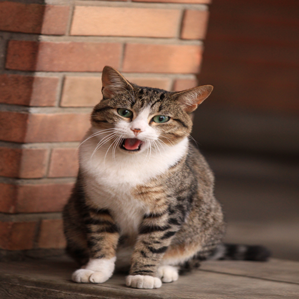
\includegraphics[width=79.62pt,height=79.62pt]{Bilder/European_cat_02_299.png}};
%Shape: Cube [id:dp48120440402395137] 
\draw  [fill={rgb, 255:red, 255; green, 255; blue, 255 }  ,fill opacity=1 ] (189,92.33) -- (149,52.33) -- (141,52.33) -- (141,171.33) -- (181,211.33) -- (189,211.33) -- cycle ; \draw   (141,52.33) -- (181,92.33) -- (189,92.33) ; \draw   (181,92.33) -- (181,211.33) ;
%Shape: Cube [id:dp1963658989292536] 
\draw  [fill={rgb, 255:red, 232; green, 232; blue, 232 }  ,fill opacity=1 ] (280,111.4) -- (241.94,73.33) -- (196,73.33) -- (196,170.27) -- (234.06,208.33) -- (280,208.33) -- cycle ; \draw   (196,73.33) -- (234.06,111.4) -- (280,111.4) ; \draw   (234.06,111.4) -- (234.06,208.33) ;
%Shape: Cube [id:dp9995029386851741] 
\draw  [fill={rgb, 255:red, 155; green, 155; blue, 155 }  ,fill opacity=1 ] (406,138.31) -- (377.08,109.4) -- (298,109.4) -- (298,171.48) -- (326.92,200.4) -- (406,200.4) -- cycle ; \draw   (298,109.4) -- (326.92,138.31) -- (406,138.31) ; \draw   (326.92,138.31) -- (326.92,200.4) ;
%Shape: Cube [id:dp47292096524654625] 
\draw  [fill={rgb, 255:red, 155; green, 155; blue, 155 }  ,fill opacity=1 ] (665.17,154.88) -- (648.62,138.33) -- (565,138.33) -- (565,173.85) -- (581.54,190.4) -- (665.17,190.4) -- cycle ; \draw   (565,138.33) -- (581.54,154.88) -- (665.17,154.88) ; \draw   (581.54,154.88) -- (581.54,190.4) ;
%Shape: Rectangle [id:dp9622310163181891] 
\draw   (736,94.33) -- (736,246.33) -- (717.17,246.33) -- (717.17,94.33) -- cycle ;
%Shape: Rectangle [id:dp3888373908322751] 
\draw   (778,104.33) -- (778,236.33) -- (759,236.33) -- (759,104.33) -- cycle ;
%Shape: Rectangle [id:dp6404657361959689] 
\draw  [fill={rgb, 255:red, 0; green, 0; blue, 0 }  ,fill opacity=1 ] (760,132) -- (776.83,132) -- (776.83,142.33) -- (760,142.33) -- cycle ;
%Straight Lines [id:da7775179037387632] 
\draw    (783.17,137.33) -- (806.17,137.33) ;
\draw [shift={(808.17,137.33)}, rotate = 180] [fill={rgb, 255:red, 0; green, 0; blue, 0 }  ][line width=0.75]  [draw opacity=0] (8.93,-4.29) -- (0,0) -- (8.93,4.29) -- cycle    ;

%Shape: Cube [id:dp25140851319063606] 
\draw  [fill={rgb, 255:red, 232; green, 232; blue, 232 }  ,fill opacity=1 ] (534.17,145.87) -- (510.63,122.33) -- (433,122.33) -- (433,172.86) -- (456.53,196.4) -- (534.17,196.4) -- cycle ; \draw   (433,122.33) -- (456.53,145.87) -- (534.17,145.87) ; \draw   (456.53,145.87) -- (456.53,196.4) ;
%Straight Lines [id:da07111443875380252] 
\draw    (189.17,135.33) -- (224.17,139.33) ;


%Straight Lines [id:da7555086779952114] 
\draw    (189.17,150.33) -- (224.17,139.33) ;


%Straight Lines [id:da6920716028952918] 
\draw    (190.17,124.33) -- (224.17,139.33) ;


%Straight Lines [id:da20921164719439567] 
\draw    (279.17,153.33) -- (314.17,157.33) ;


%Straight Lines [id:da5314884265558493] 
\draw    (279.17,168.33) -- (314.17,157.33) ;


%Straight Lines [id:da9607824424543641] 
\draw    (280.17,142.33) -- (314.17,157.33) ;


%Straight Lines [id:da22420538027937398] 
\draw    (405.17,162.33) -- (440.17,166.33) ;


%Straight Lines [id:da8064502796691653] 
\draw    (405.17,177.33) -- (440.17,166.33) ;


%Straight Lines [id:da9671090843658954] 
\draw    (406.17,151.33) -- (440.17,166.33) ;


%Straight Lines [id:da6406059045755481] 
\draw    (533.17,166.33) -- (568.17,170.33) ;


%Straight Lines [id:da9716418537016991] 
\draw    (533.17,181.33) -- (568.17,170.33) ;


%Straight Lines [id:da548327903780097] 
\draw    (534.17,155.33) -- (568.17,170.33) ;


%Straight Lines [id:da32303530471950226] 
\draw    (665.17,171.33) -- (715.17,171.33) ;
\draw [shift={(717.17,171.33)}, rotate = 180] [fill={rgb, 255:red, 0; green, 0; blue, 0 }  ][line width=0.75]  [draw opacity=0] (8.93,-4.29) -- (0,0) -- (8.93,4.29) -- cycle    ;

%Straight Lines [id:da4465574217797632] 
\draw    (735.17,171.33) -- (757.17,171.33) ;
\draw [shift={(759.17,171.33)}, rotate = 180] [fill={rgb, 255:red, 0; green, 0; blue, 0 }  ][line width=0.75]  [draw opacity=0] (8.93,-4.29) -- (0,0) -- (8.93,4.29) -- cycle    ;

%Shape: Rectangle [id:dp05899425458959939] 
\draw  [color={rgb, 255:red, 160; green, 160; blue, 160 }  ,draw opacity=1 ][fill={rgb, 255:red, 160; green, 160; blue, 160 }  ,fill opacity=1 ] (760,203) -- (776.83,203) -- (776.83,213.33) -- (760,213.33) -- cycle ;
%Straight Lines [id:da9780199762846196] 
\draw    (784.17,206.33) -- (807.17,206.33) ;
\draw [shift={(809.17,206.33)}, rotate = 180] [fill={rgb, 255:red, 0; green, 0; blue, 0 }  ][line width=0.75]  [draw opacity=0] (8.93,-4.29) -- (0,0) -- (8.93,4.29) -- cycle    ;


% Text Node
\draw (840,135) node  [align=left] {Cat \ $\displaystyle 0.8$};
% Text Node
\draw (185,219) node  [align=left] {$\displaystyle 3$};
% Text Node
\draw (153,199) node [rotate=-45.72] [align=left] {$\displaystyle 299$};
% Text Node
\draw (131,111) node [rotate=-269.52] [align=left] {$\displaystyle 299$};
% Text Node
\draw (235,54) node  [align=left] {Convolution};
% Text Node
\draw (339,89) node  [align=left] {Pooling};
% Text Node
\draw (609,119) node  [align=left] {Pooling};
% Text Node
\draw (724,72) node  [align=left] {Dense};
% Text Node
\draw (770,86) node  [align=left] {Dense};
% Text Node
\draw (690,184) node  [align=left] {Flatten};
% Text Node
\draw (477,103) node  [align=left] {Convolution};
% Text Node
\draw (145,35) node  [align=left] {Input};
% Text Node
\draw (841,204) node  [align=left] {Dog \ $\displaystyle 0.1$};


\end{tikzpicture}